%%%%%%%%%%%%%%%%%%%%%%%%%%%%%%%%%%%%%%%%%%%%%%%%%%%%%%%%%%%%%%%%%%%%%%%%%%%%%%%%
%2345678901234567890123456789012345678901234567890123456789012345678901234567890
%        1         2         3         4         5         6         7         8

\documentclass[letterpaper, 10 pt, conference]{ieeeconf}  % Comment this line out if you need a4paper
\usepackage[colorlinks,linkcolor=black]{hyperref}

%\documentclass[a4paper, 10pt, conference]{ieeeconf}      % Use this line for a4 paper

\IEEEoverridecommandlockouts                              % This command is only needed if
                                                          % you want to use the \thanks command

\overrideIEEEmargins                                      % Needed to meet printer requirements.

%In case you encounter the following error:
%Error 1010 The PDF file may be corrupt (unable to open PDF file) OR
%Error 1000 An error occurred while parsing a contents stream. Unable to analyze the PDF file.
%This is a known problem with pdfLaTeX conversion filter. The file cannot be opened with acrobat reader
%Please use one of the alternatives below to circumvent this error by uncommenting one or the other
%\pdfobjcompresslevel=0
%\pdfminorversion=4

% See the \addtolength command later in the file to balance the column lengths
% on the last page of the document

% The following packages can be found on http:\\www.ctan.org
\usepackage{amsmath} % assumes amsmath package installed
\usepackage{amssymb}  % assumes amsmath package installed

\usepackage{amsfonts}
\usepackage{cite}
\usepackage[ruled,vlined]{algorithm2e}
\usepackage{graphicx}
\usepackage{subcaption}% needed for subfigure
\usepackage{diagbox}
%\usepackage{biblatex}
%\usepackage{textcomp}
\usepackage{xargs}
\usepackage[pdftex,dvipsnames,table]{xcolor}
\usepackage{dirtree}
\usepackage{multirow}
\usepackage{verbatim}
\title{\LARGE \bf
SUSTech POINTS: A Portable 3D Point Cloud Interactive Annotation Platform System

}

\author{E Li$^{1}$,Shuaijun Wang$^{1,2}$,  Chengyang Li$^{1}$, Dachuan Li$^{1}$,Xiangbin Wu$^{3}$, and Qi Hao$^{1,*}$% <-this % stops a space
\thanks{This work is partially supported by the National Natural Science Foundation of China (No: 61773197), the Science and Technology Innovation Committee of Shenzhen City (No: GJHZ20170314114424152), the Nanshan District Science and Technology Innovation Bureau (No: LHTD20170007), and the Intel ICRI-IACV Research Fund (CG$\#$52514373).}
\thanks{$^{*}$Corresponding author: Qi Hao (hao.q@sustech.edu.cn).}
\thanks{$^{1}$Department of Computer Science and Engineering,
Southern University of Science and Technology, Shenzhen, Guangdong, China, 518055}
\thanks{$^{2}$Harbin Institute of Technology,
92 West Dazhi Street, Nan Gang District, Harbin, China, 150001}%
% <-this % stops a space
\thanks{$^{3}$Intel Chinese Research Institute-Intelligent \& Automated Connected Vehicles}%
% <-this % stops a space
}


\begin{document}
\maketitle
\thispagestyle{empty}
\pagestyle{empty}
%%%%%%%%%%%%%%%%%%%%%%%%%%%%%%%%%%%%%%%%%%%%%%%%%%%%%%%%%%%%%%%%%%%%%%%%%%%%%%%%
\begin{abstract}

The major challenges of developing 3D point cloud annotation systems for autonomous driving datasets include
convenient user-data interfaces, efficient operations on geometric data units, and scalable annotation tools. 
This paper presents a {Portable pOint-cloud Interactive aNnotation plaTform System} (i.e. SUSTech POINTS), 
which contains a set of user-friendly interfaces and efficient annotation tools to help achieve high quality data annotations with high efficiency. 
The novelty of this work includes threefolds: 
(1) developing a set of visulization modules for fast annotation error localization and convenient annotator-data interactions; 
(2) developing a set of interactive tools for annonators labelling 3D point clouds and 2D images in high speeds;
(3) developing an annotation transfer method to label the same objects in different data frames. 
The developed POINTS system is tested with public datasets such as KITTI and a private dataset (SUSTech SCAPES). 
The experiment results show that the developed platform can help improve the annotation accuracy and efficiency pretty much 
compared with using other open-source annotation platforms.



\end{abstract}


%%%%%%%%%%%%%%%%%%%%%%%%%%%%%%%%%%%%%%%%%%%%%%%%%%%%%%%%%%%%%%%%%%%%%%%%%%%%%%%%




\section{Introduction}


Building accurately annotated autonomous driving (AD) datasets is critical for training and verification of situation perception and data fusion algorithms. 
While 3D points clouds can provide high-accuracy geometric relations among the ego-vehicle, surrounding objects and the environment, 
2D images contain high-resolution information of objects and the environment. 
Recent AD datasets take advantages of high-resolution, multi-perspective 2D data to improve the annotation quality of 3D data 
based on their underlying correlations. 
There are three major components for intelligent AD dataset annotation systems: 
(1) data pre-processing, (2) data visualizations, and (3) interactive operations, 
which are enabled by a data management system and a user-data interaction interface, as shown in Fig.~\ref{fig:main-arch}.

Despite many efforts and successes in developing AI-based pre-processing techniques, data visualizations and interactive operations also impose a number of technical challenges upon developing an efficient data annotation platform, including
\begin{enumerate}

\item \textbf{Fast Error Checking}. Given the initial annotation results of 2D and 3D data, it is required to develop a set of data visualizaton modules that can help annotators quickly localize those annotation errors. 
\item \textbf{Easy user-data interactions}. Each frame of data usually contains a great number of objects with irregular measurement data in a large field of view (FOV), hence it is necessary to develop a convenient human-computer interface to enable annotators to easily perform corrective operations upon annotation errors.
\item \textbf{Flexible annotation extension}. There are a lot underlying correlations among data frames, FOVs, and sensing modalities, so the annotations of the same objects should be scalable and extensible among different frames, areas and modalities.

\end{enumerate}




\begin{figure}[tp]
	\centering
	% Requires \usepackage{graphicx}
	%\resizebox{\linewidth}{!}{
	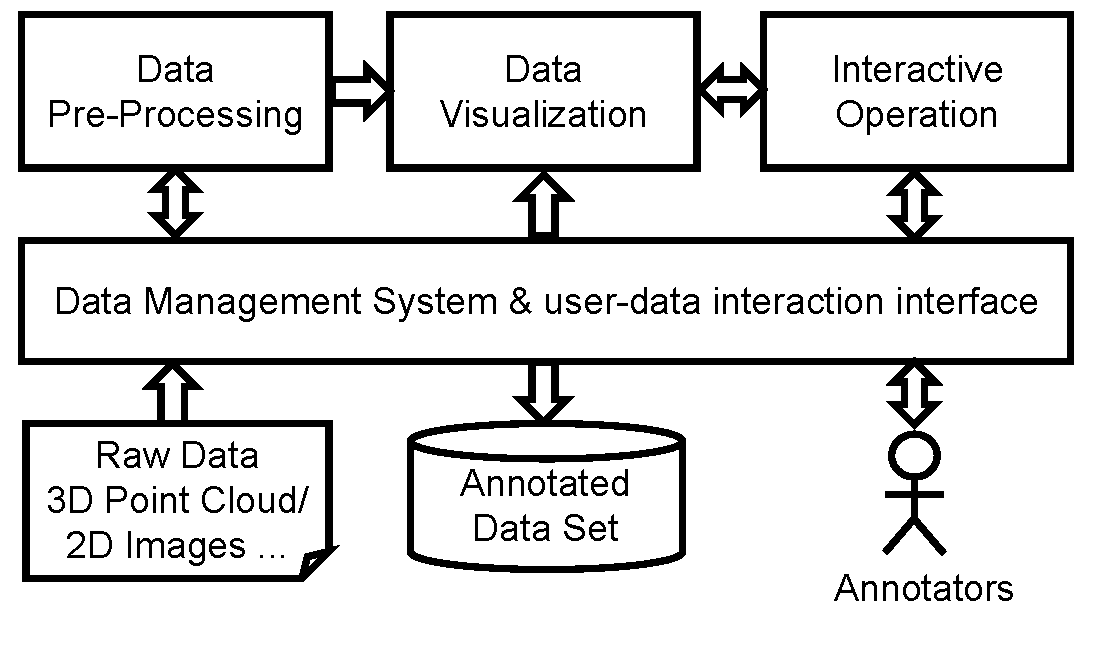
\includegraphics[width=0.45\textwidth]{./platform-simple2}\\ %\vspace{-0.3cm}
	\caption{An illustration of intelligent annotation systems for autonomous driving datasets.}
	\label{fig:main-arch}
	\vspace{-0.3cm}
\end{figure}




\begin{table*}[h]
	\caption{A comparison of 3D point cloud annotation systems in terms of visualization modules and interactive operations}
	\label{tab:comparison}
	\resizebox{1.0\textwidth}{!}{
		\begin{tabular}{c||p{1.1cm}<{\centering}|p{0.7cm}<{\centering}|p{1cm}<{\centering}|p{1cm}<{\centering}|p{1cm}<{\centering}|p{0.9cm}<{\centering}|p{1cm}<{\centering}|p{0.7cm}<{\centering}|p{1cm}<{\centering}
				||p{1cm}<{\centering}|p{1cm}<{\centering}|p{0.9cm}<{\centering}|p{1cm}<{\centering}|p{1cm}<{\centering}}
			\hline \hline
			\multirow{2}{*}{} & \multicolumn{9}{c||}{Visualization}                         & \multicolumn{5}{c}{Operation}                 \\
			\cline{2-15}                       &3D Spatial/ Temporal Navigation & Main View Focus Mode   & Box \& Object Coloring & Top/Side/ Front Views  &Photo Context with 3D-2D Fusion  &Focused Context & Mult-Camera Switching & Stream Play & Object Locking    & Box Degrees of Freedom & Auto Box Initialization& Sub-View Editing &Interactive Box Fitting  & Annotation Transfer \\  \hline
			PointAtMe~\cite{pointatme}         &                 $\surd$  & $\times$               &  $\times$              &  n/a                     & $\surd$*                        &  $\times$      &  $\times$                       &  $\times$    &  $\times$                       & 9                      &     -                    &   n/a            &   -                 &   -            \\ \hline
			3D BAT~\cite{Zimmer20193DBA}       &                 $\surd$  & $\times$               &  $\surd *$             &  $\surd$*              & $\surd$                         &  $\times$      &  $\surd$*                       &  $\times$    &  $\times$                       & 9                      &     -                    &   -              &   -                 &   ++            \\ \hline
			LATTE~\cite{Wang2019LATTEAL}       &                 $\surd$  & $\times$               &  $\times$              &  $\times$              & $\surd$*                        &  $\times$      &  $\times$                       &  $\times$    &  $\times$                       & 5                      &     ++                   &   -              &   -                 &   ++            \\ \hline
			Supervise.ly~\cite{SUPERVISELY}    &                 $\surd$  & $\times$               &                        &  $\surd$               & $\surd$                         &  $\times$      &  $\times$                      &              &                                 & 9                      &     -                    &   ++             &   -                 &                  \\ \hline
			scale.ai~\cite{scale}              &                 $\surd$  & $\times$               &  $\surd *$             &  $\surd$               & $\surd$                         &  $\times$      &  $\surd$*                       &              &                                 & 7                      &                          &                  &   -                 &                 \\ \hline
			Playment.io~\cite{Playment}        &                 $\surd$  & $\times$               &  $\surd *$             &  $\surd$               & $\surd$                         &  $\times$      &  -                              &  $\surd*$    &  $\surd$                        & -                      &     -                    &   ++             &   -                 &   ++            \\ \hline
			\textbf{Ours (POINTS)}                      &                 $\surd$  & $\surd$                &  $\surd$               &  $\surd$               & $\surd$                         &  $\surd$       &  $\surd$                        &  $\surd$    &  $\surd$                        & 9                      &     +++                  &  +++             &  +++                &  +++            \\ \hline \hline
		\end{tabular}
	}
	\begin{tabular}{p{17.5cm}}
		
		
		The symbol ``$\surd$'' means that the system supports the functionality, ``$\times$'' means does not support,  and ``$\surd$*'' means partially supports. 
		The number of ``$\textbf{+}$''s represents the performance of a specific funcationality, more ``$\textbf{+}$''s means better performance, and ``-'' means a lack of that functionality. Some functionalities are explained as below:

		\begin{enumerate}
			\item ``Main View Focus Mode'': to zoom in and center a selected object in the main view with one click.
			
			\item ``Stream Play'': to play the sequential 3D data as a video stream
			
			\item ``Object Locking'': to automatically select the same object in all frames when the stream is playing.
			
			\item ``Focused Context'': to display the 2D image of the current object as a photo context in a single sub-view
			
			\item ``Camera Auto-Switching'': to automatically switch the photo context among multiple cameras when navigating objects.
			
			\item ``Auto Box Initialization'': to automatically fit the 3D annotation box to the whole 3D object data with one click on one point of the object data.
			
			\item ``Sub-View Editing'': to edit the 3D annotation box in one of the projective sub-views.
			
			\item ``Interactive Box Fitting'': to automatically fit the 3D annotation box to the 3D object data when editing (e.g. rotating, translating, and resizing).
			
			\item ``Annotation Transfer'': to transfer annotations across frames by an automatic or semi-automatic way.
			
		\end{enumerate}
		The meaning of other functionalities could be understood by their own names.
		
		
		
		% after \\: \hline or \cline{col1-col2} \cline{col3-col4} ...
	\end{tabular}
	\label{tab:annotationMethods}
	\vspace{-0.5cm}
\end{table*}




Current AD dataset annonation systems have developed temporal and spatial navigation tools to help quickly review annotation results \cite{Playment,SUPERVISELY,Wang2019LATTEAL,Zimmer20193DBA}, 
assigning different colors to annotation boxes to distinguish objects \cite{SUPERVISELY,Zimmer20193DBA,Playment,scale}, 
providing various perspective/projective views and multi-camera photo contexts of 3D data to help localize annotation errors \cite{SUPERVISELY,Playment,Zimmer20193DBA}, 
and supporting data stream playing and object locking in data streams to help check out the temporal consistency ammong annotation results \cite{Playment}.
However, more visualization modules such as background removal, object based coloring, and modality/spatial/temporal consistency checking should be further developed to improve the error checking efficiency.
On the other hand, interactive operations such as high degrees-of-freedom (DOFs) and multi-view editing, box initalization (one-click annotation)
and automatic fitting have also been developed \cite{pointatme,Zimmer20193DBA,Wang2019LATTEAL,SUPERVISELY,Playment}; but all need further refinement to increase annotation efficiency. 
Besides, several annotation transfer methods have been developed to achieve annotation extensions to multiple frames \cite{Playment,Wang2019LATTEAL,Zimmer20193DBA}, 
but no registration-based method has been proposed yet, which can provide more accuracy and higher speeds for annotations.


In this paper, we present a comprehensive web-based AD dataset annotation platform system, which provides more advanced functionalities in visualization modules, interactive tools, and annotation trasnfer. The contributions of this work include
\begin{enumerate}
	\item developing an open-source portable 3D point cloud annotation platform with well-designed visualization modules and high-efficiency interactive tools, whose source codes are available for public access on Github (\url{https://github.com/naurril/SUSTechPOINTS}).
	\item developing a series of enhanced data visulization modules such as stream playing, object locking, background removal, object based coloring, multi-camera
swiching, and photo context adjusting to enable fast error checking.
	\item developing a series of new interactive tools such as smart box initialization and interactive box fitting to enable fast and accurate 3D data annotating.
	\item developing a novel registration-based inter-frame annotation transfer method, which can extend annotation results from one frame to the whole data stream with high accuracy and speeds.

\end{enumerate}


%%The platform is available for public access on github\footnote{ https://github.com/naurril/SUSTechPOINTS}.

The rest of this paper is organized as follows. 
Section~\ref{sec:realtedwork}  reviews the state-of-the-art AD dataset annotation systems and highlights the novelty of our system. 
Section~\ref{sec:systemarch} describes the system architecture and major functionalities of the proposed POINTS system. 
Section~\ref{sec:results} provides the experiment results and related discussions. 
Section~\ref{sec:conclusions} concludes the paper and outlines future work.





\begin{figure*}[t]
	
	\centering
	\vspace{-0.1cm}
	% Requires \usepackage{graphicx}
	%\resizebox{\linewidth}{!}{
	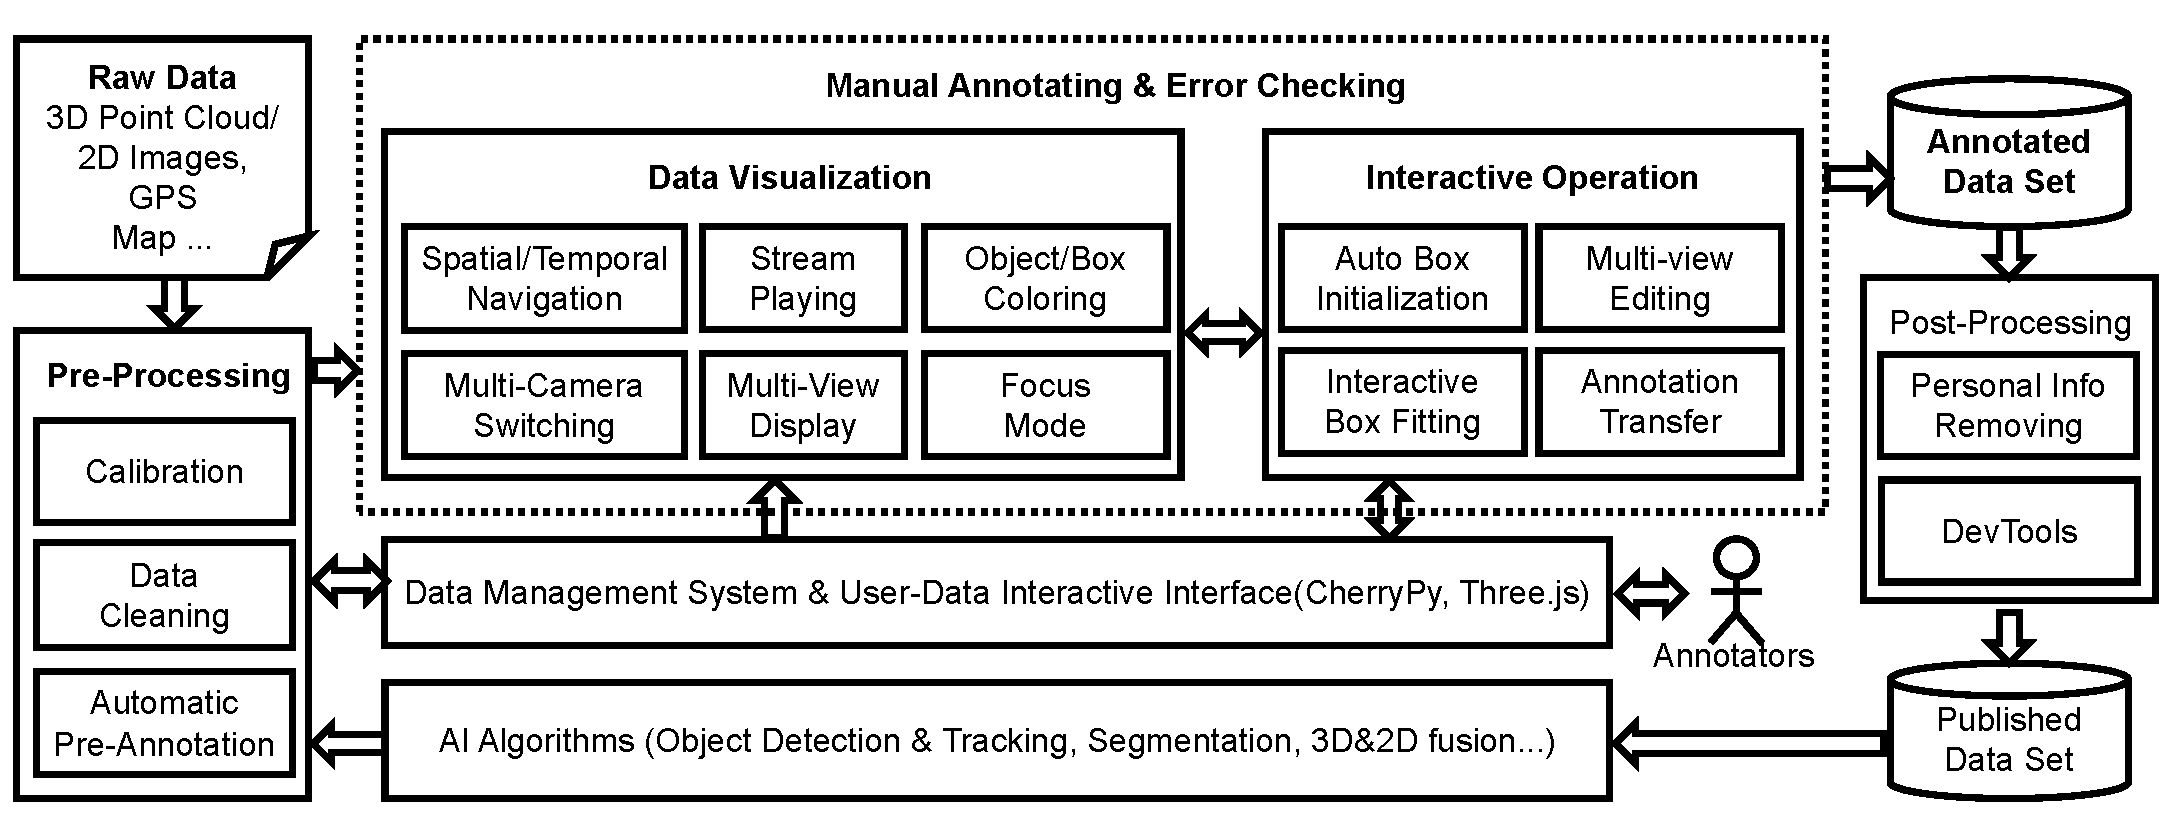
\includegraphics[width=1.0\linewidth]{./arch-big}\\ %\vspace{-0.3cm}
	\caption{The system architecture of the proposed portable point cloud interactive annotation platform system (POINTS).}
	\label{fig:arch_layer}
\end{figure*}


\section{Related work}
\label{sec:realtedwork}



Table~\ref{tab:comparison} summarizes a detailed comparison of the most popular 3D point clouds annotation systems in terms of visualization modules and interactive operations, where the first 3 systems (PointAtMe\cite{pointatme}, 3D BAT\cite{Zimmer20193DBA}, LATTE\cite{Wang2019LATTEAL}) and ours (POINTS) are open-source software, 
and the remainning 3 systems (Supervise.ly\cite{SUPERVISELY}, scale.ai\cite{scale}, Playment.io\cite{Playment}) are commercial platforms. 
It can be seen that in general the commercial platforms can provide advanced functionalities of data visualizations and interative operations, 
but their technological details are undisclosed. 
By comparison, our open-source annotation platform (POINTS) can provide unique functionalies of main view focus mode, focused context and interactive box fitting, plus more advanced functionalities of stream playing, object locking, sub-view editing, auto box initialization and annotation transfer.

3D point cloud annotation systems can be classified as screen based and virtual-reality (VR) based. 
In the screen based systems, point clouds are visualized on 2D computer screens; users annotate objects by drawing 3D boxes with
keyboads, mouse devices and/or gestures (if touch screens are available) \cite{LabelMe3D}; camera images are displayed to help identify objects; various algorithms are developed to assist iteractive operations \cite{Wang2019LATTEAL}. 
VR based systems can provide better immersive experiences for users\cite{pointatme, gothentag}, but suffer from limits such as inaccurate operations and motion sickness. 
Therefore, in this work we choose a screen based interface to develop our annotation system.

Annotation systems can also be classified as web-based and PC-based. 
The web-based systems, such as 3D-BAT\cite{Zimmer20193DBA} and supervise.ly \cite{SUPERVISELY}, are portable for users to perform 3D object annotations only using web browsers. 
The PC-based systems, such as AppoloSuite \cite{wang2019apolloscape}, need software installed to perform annotations. 
As a result, these systems need to be updated from time to time and annotation datasets need to be downloaded from servers. 
Our proposed POINTS system is web-based, enabled by the CherryPy \cite{cherrypy} web application development framework. 
We believe that web-based systems are more portable and scalable for massive data annotating when many annotators are involved.

There are no standard benchmark metrics for annotation system evaluation yet, to the best of our knowledge.
Annotation efficiency can be measured by the annotation time used by annotators \cite{monica2017multi,pointatme,Zimmer20193DBA}. 
PointAtMe evaluates the annotation accuracy by using labor-intensive annotation results as the ground truth \cite{pointatme}. 
In this work, we choose the metrics used by PointAtMe \cite{pointatme} to evalute the efficiency and accuracy of our developed tools, 
and use its experiment results as the baseline to compare with.


\section{System Architecture and Module Functionalities}
\label{sec:systemarch}

\subsection{System Architecture}

The web-based POINTS focuses on developing visualization modules and interative tools for 3D bounding box and tracking ID annotation.
The platform web server manages all the data, programmed with the CherryPy \cite{cherrypy} web application development framework.
The platform fronend provides almost all the module functionalities, programmed with the \texttt{WebGL} library Three.js \cite{threejs}.
Fig.~\ref{fig:arch_layer} shows the system architecture of POINTS.
In the data pre-processing stage, intrinsic/extrinsic sensor parameters are estimated first; only those data frames consistent to calibration parameters, useful for algorithms training and verification are selected; then a set of AI algorithms including detection, segmentation, and 2D\&3D fusion are used to annotate the dataset initially. The data visualization modules provide helpful temporal/spatial navigation tools for users, distinguish data of different objects, and show multiple views of each object from different perspectives. The interactive data operations include editing labels in multiple views, automatically adjusting the size of 2D/3D boxes to fit the data of each object, and automatically extending (transferring) annotations of the same objects from one frame (modality) to different frames (modalities).

\subsection {Data Visualization Modules}
\label{sec:visualization}
\begin{figure}[!t]
	\centering	
	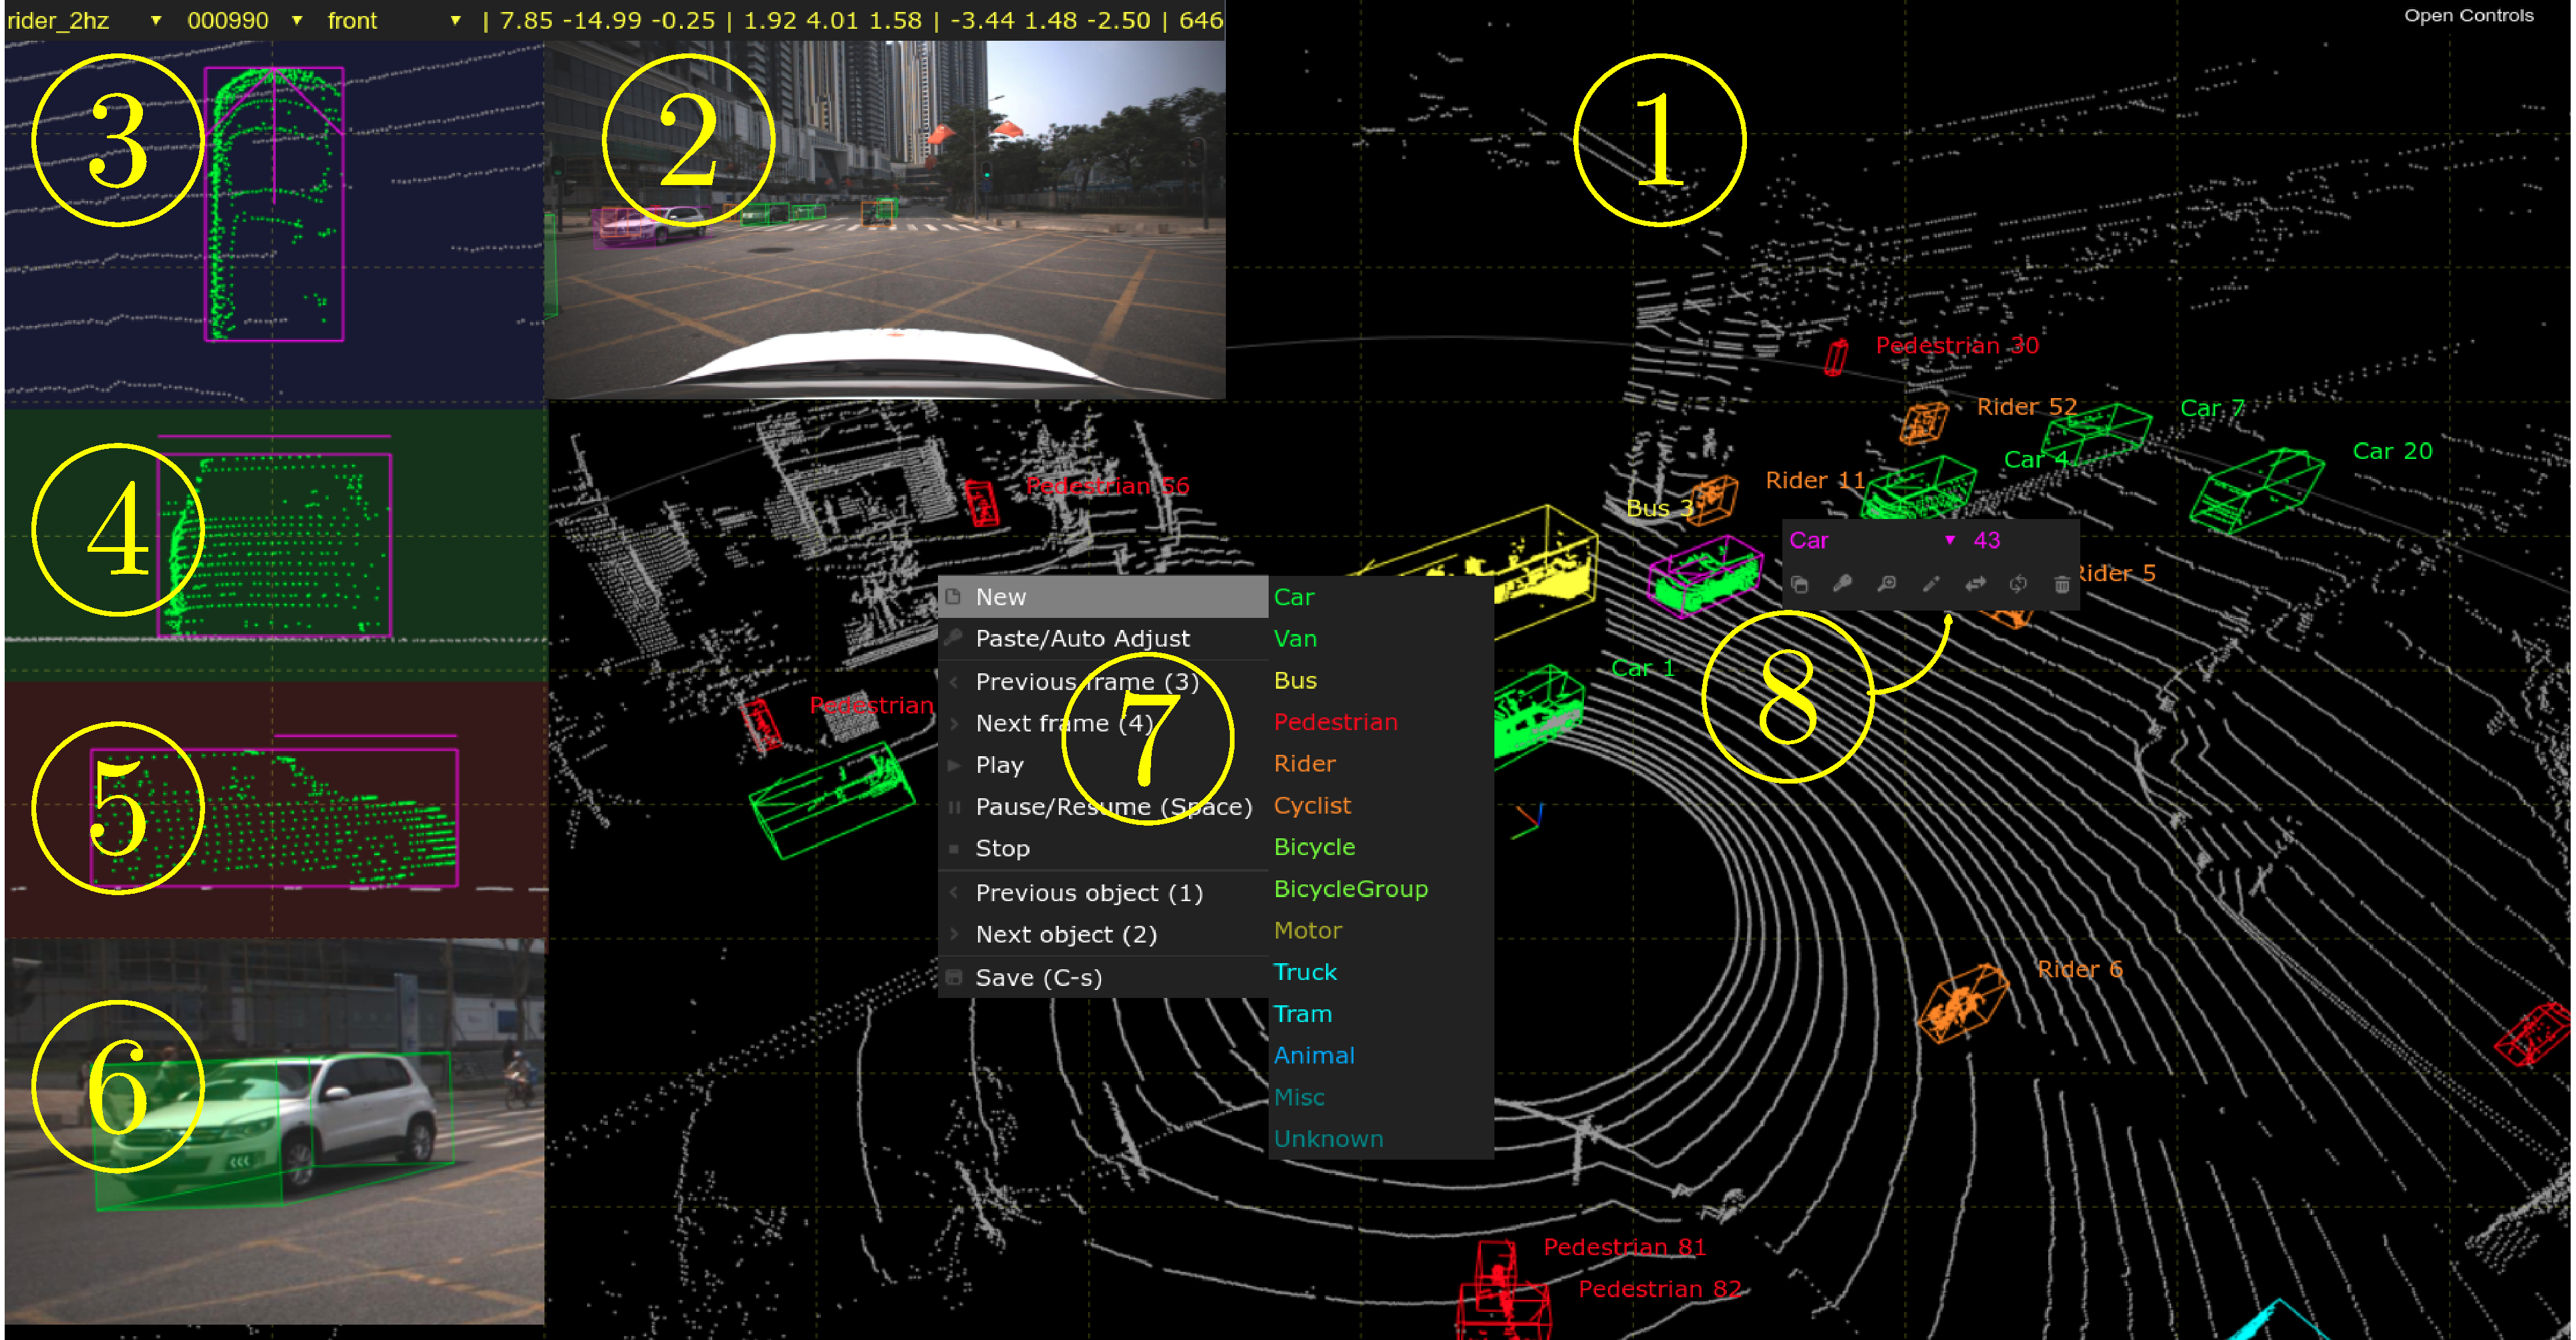
\includegraphics[width=\linewidth]{./figures/main-ui}\\
	\caption{The main UI of POINTS. 
		\textcircled{1} the perspective view of the 3D point cloud; 
		\textcircled{2} the photo context, which is resizable and can be automatically switched among multiple camera images; 
		\textcircled{3} the top view of the selected object;
		\textcircled{4} the front view of the selected object; 
		\textcircled{5} the side view of the selected object; 
		\textcircled{6} the focused photo context, which can be automatically chosen for the selected object ;
		\textcircled{7} the context menu, which provides tools of context operations; 
		\textcircled{8} the floating fast toolbox, which provides most used tools.}
	\label{fig:main-ui}
\end{figure}


Data visualization modules help edit and review the annotation results in terms of 3D boxes. 
Fig.~\ref{fig:main-ui} shows the main user interface (UI) of POINTS, from which all the visualization functionalities can be achieved.
The main UI contains the following functionalites: 
\textbf{Sub-views}. The main window is divided into one main view (\textcircled{1} in Fig.~\ref{fig:main-ui}) and five sub-views,  and the top, front and side projective views of the selected object are displayed on the left side (\textcircled{3},\textcircled{4},\textcircled{5} in Fig.~\ref{fig:main-ui})with the background hidden. The context photo of the selected object is displayed in the top middle sub-view (\textcircled{2} in Fig.~\ref{fig:main-ui}) and an extra focused context is displayed in the bottom left sub-view (\textcircled{6} in Fig.~\ref{fig:main-ui}); the 3D annotation box of the selected object is projected onto these two sub-views.
\textbf{Focus-mode}. A focus mode is provided to help check the details of the selected object. When the mode is activated through the fast toolbox (\textcircled{8}) in Fig.~\ref{fig:main-ui}), the selected object will be automatically centered in the main view and zoomed in with most of the background hidden.
\textbf{Camera auto-switching}. Multiple camera images can be all displayed on the top of the main view \cite{Zimmer20193DBA}, or only one of them displayed to provide more focus \cite{scale,Wang2019LATTEAL,pointatme}, which requires automatic switching to the most relevant camera for a selected object. Manual camera selection should also be provided. Note that this functionality needs accurate calibration parameters of sensors.
\textbf{Object coloring}. All boxes and points can be colored by their categories. A selected object will be highlighted with a different color. 
\textbf{Navigation}. \label{sec:navigation} A user can quickly check the annotation results in the 3D space, or along the time axis, by changing the point of view, selected objects and the no. of frames.
\textbf{Stream play}. \label{sec:streamplay} A user can play the sequential data in terms of scenes like a video.
\textbf{Object locking}. When a data stream is playing, a selected object can be locked, highlighted with a specific color, in all frames.
\textbf{Box information}. The detailed information (scene, frame, object category, coordinates, dimension, orientation and the number of points) of each selected box will be displayed on the top of the main window.

\subsection{Interactive Operations: 3D Box Tools}
\begin{figure}[t]
	\centering
	\resizebox{\linewidth}{!}{
		\begin{subfigure}{0.3\linewidth}
			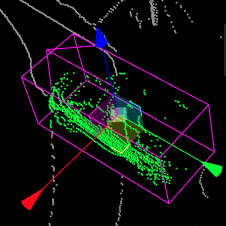
\includegraphics[height=2.5cm]{./figures/box-move}
			\caption{Translation}
		\end{subfigure}
		\begin{subfigure}{0.3\linewidth}
			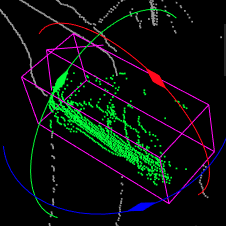
\includegraphics[height=2.5cm]{./figures/box-rotate}
			\caption{Rotation}
		\end{subfigure}	
		\begin{subfigure}{0.3\linewidth}
			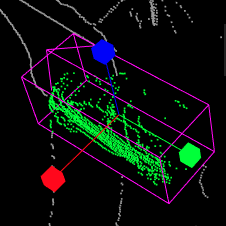
\includegraphics[height=2.5cm]{./figures/box-resize}
			\caption{Scaling}
		\end{subfigure}
	}
	\caption{An illustration of annotaton box operations in the perspective view.}
	\label{fig:box-mouse-edit}
\end{figure}
\begin{figure}[t]
	\centering
	\resizebox{\linewidth}{!}{
		\begin{subfigure}{0.3\linewidth}
			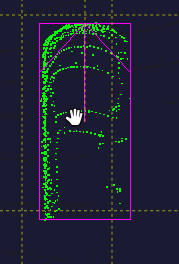
\includegraphics[height=4.cm]{./figures/subview-move-xy}
			\caption{Translation}
		\end{subfigure}
		~
		\begin{subfigure}{0.3\linewidth}
			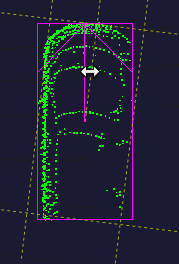
\includegraphics[height=4.cm]{./figures/subview-rotate-xy}
			\caption{Rotation}
		\end{subfigure}
		~
		\begin{subfigure}{0.3\linewidth}
			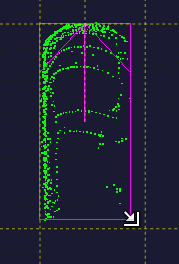
\includegraphics[height=4.cm]{./figures/subview-resize-xy}
			\caption{Scaling}
		\end{subfigure}	
	}
	\caption{An illustration of annotation box operations in the top projective view. Dotted lines suggest the next box pose after each operation.}
	\label{fig:box-mouse-edit-subview}
\end{figure}
\textbf{3D box intialization}. A user can create a new 3D box by right clicking on an object and then select the object type from the popup context menu. 
Our platform performs the following functionalities to help create a box easily:
1) The initial box oritation is upward (\textit{i}.\textit{e} the degree of yaw along the z-axis is zero) within the main view of the x-y plane.  
2) A box prototype (in accordance with the object type) is placed at the position of the mouse pointer.
3) A Euclidean distance based growing algorithm is invoked to estimate all the points belonging to the object.
4) An auto-fitting algorithm (Section~\ref{sec:support-algorithms}) is used to shrink the box size in case there is a margin between the box and the points of the object.

Note that in most cases, the annotation can be completed with such a single click. Different from the one-click-annotation of LATTE \cite{Wang2019LATTEAL}, which uses a clustering algorithm to search the points belonging to the object under selection, our method uses box prototypes to overcome numerical difficulties when the points of an object is too sparse for clustering algorithms. A user can also create a new box by drawing a 2D rectangle within the main view, enclosing relevant points. The box is initialized by setting its orientation as above and automatically fitted to the enclosed points. The object type is automatically chosen by simply matching the dimension of the object with those of prototypes.

\textbf{3D box editing in the perspective view}. When an object is selected, a floating fast toolbox will appear next to it, as shown in Fig.~\ref{fig:main-ui}. A user can change the object type, tracking id, activate the focus mode, among others. For tracking ID, a user can input or select existing value in the fast toolbox, or select `auto' option letting the platform to generate a unique new ID  in the scene. A user can click on an object or the button of the fast toolbox to enable box editing, and drag the handlers to resize, rotate or translate the box, as shown in Fig.~\ref{fig:box-mouse-edit}. Corresponding keyboard shortcuts are also provided.
\textbf{3D box editing in the projective sub-views}. Editing a 3D box in the perspective view is inconvenient as the user has to change the viewpoint from time to time. As shown in Fig.~\ref{fig:main-ui}, the annotation results are more clearly displayed in the projective sub-views,  hence our platform enables the user to rotate, resize or translate the box in the projective subviews by using mouse operations, as shown in Fig.~\ref{fig:box-mouse-edit-subview}. All operations can also be done with keyboard shortcuts.



\subsection{Interactive Operations: Supporting Algorithms}
\label{sec:support-algorithms}

\begin{figure}[t]
	\centering
	
	\begin{subfigure}[t]{0.18\linewidth}
		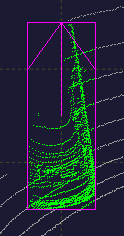
\includegraphics[height=3cm]{./figures/rotation-begin}
		\caption{}
		\label{fig:box-before-rotate}
	\end{subfigure}\hfill
	\begin{subfigure}[t]{0.18\linewidth}
		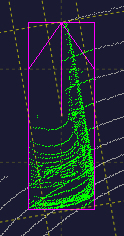
\includegraphics[height=3cm]{./figures/rotation-dotted-lines}
		\caption{}
		\label{fig:box-rotate-in-subview}
	\end{subfigure}\hfill
	\begin{subfigure}[t]{0.18\linewidth}
		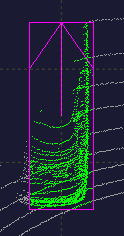
\includegraphics[height=3cm]{./figures/rotation-fail-points-go-out}
		\caption{}
		\label{fig:box-rotate-naively}
	\end{subfigure}\hfill
	\begin{subfigure}[t]{0.18\linewidth}
		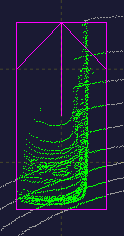
\includegraphics[height=3cm]{./figures/rotation-fail-by-ground-plane}
		\caption{}
		\label{fig:box-rotate-fail-by-ground}
	\end{subfigure}\hfill
	\begin{subfigure}[t]{0.18\linewidth}
		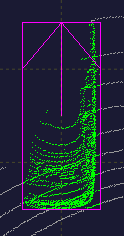
\includegraphics[height=3cm]{./figures/rotation-succeeded}
		\caption{}
		\label{fig:box-rotate-correctly}
	\end{subfigure}\hfill
	\caption{ 
		An illustration of box auto-fitting after rotation. (a) A bounding box enclosing all points of a car. (b) A counter-clockwise rotation of the bounding box. (c) Part of the points of the car going outside the bounding box without auto-fitting. (d) Auto-fitting of the bounding box to the points of the car, where the final bounding box becomes a little bit larger than the car because of the presence of ground points (circular arcs). (e) Auto-fitting of the bounding box to the points of the car, with the ground plane problem solved by our algorithm,  the bounding box fits the object well.}
	\label{fig:boundary-aware-rotation}
	\vspace{-0.3cm}
\end{figure}



\textbf{Interactive box fitting}. 
When a bouding box is resized or rotated, our platform can fit the box to the object automatically by finding the minimal box enclosing all the points of the object. Fig.~\ref{fig:boundary-aware-rotation} illustrates the process of box auto-fitting after rotation; as the result, all the points of the car are kept inside the bounding box. 
With this functionality, only two steps are needed to annotate a new object: (1) draw a rectangle to enclose all the pionts of an object; (2) rotate the 3D bounding box once. Note that the algorithm to find the minimal box may fail when the points of ground are present. 
For example, in Fig.~\ref{fig:box-rotate-fail-by-ground}, because the ground points (circular arcs) are present, the auto-fitted box becomes a little bit larger than the object. 
One possible solution is to remove the ground points using algorithms, but it is not reliable when the ground is not smooth (as often can be seen in the KITTI dataset \cite{Geiger2012CVPR} where cars are often parked across the curb (Fig.~\ref{fig:annocheck})). We use a simple but effective method to solve this problem. Specifically, a large part  of the object bottom  (0.2m along the z-axis by default) is skipped while the object size along x-y dimensions (width and length) are accurately estimated, such that the ground points can be removed effectively. In real-world traffic scenarios, almost all objects are much higher than 0.2m. After such a object size estimation, the reduced 0.2m will be compensated along the z-dimension (height). The Interactive Box Fitting algorithm is summarized in Algorithm~\ref{alg:box-fitting}.

\begin{algorithm}
	\caption{Interactive Box Fitting Algorithm.}
	\label{alg:box-fitting}
	
	\SetAlgoLined
	\KwIn{point cloud $\mathcal{P} \in \mathbb{R}^{n \times 3}$; original box $b=(p, s, r)$; operation $o = (r',s')$, where $p,s,r \in \mathbb{R}^3$ means  position, scale and rotation, respectively, rotation is represented by Euler angles, $r',s'$ means rotating angles and scale changes of the operation $o$.}
	\KwOut{box $b'$ after operation.}
	\nl find all points $\mathcal{R}$ inside box $b$\;
	\nl construct coordinate system $B'$ with original point $p$ and axes angles $r+r'$\;
	\nl construct range $c$ by applying $s'$ on $s$, represented as $x,y,z$ coordinate ranges\;
	\nl compute $\mathcal{P'}$ by representing $\mathcal{P}$ in coordinate system $B'$\;
	\nl initialize $\mathcal{R'} = \emptyset$\;
	\For{point $x$ in $\mathcal{P'}$}{
		\If{$x$ is in $\mathcal{R}$}{add $x$ into $\mathcal{R'}$}
		\ElseIf{$x$ is in range $c$ }{add $x$ into $\mathcal{R'}$}
		}
	\nl compute coordinates range $d$ of $\mathcal{R'}$ by finding maximum and minimum values along each coordinate axis. when computing $x,y$ ranges, ignore points whose $z$ value is in the lowest 0.2m part\;
	\nl compute position delta $\delta p$ and scale $s''$ of new box $b'$ in coordinate system $B'$ by range $d$\;
	\nl compute $\delta p'$ by reprensenting $\delta p$ in original coordinate system of $\mathcal{P}$
	
	\nl return $b' = (p+\delta p', s'', r+r')$\;
	
\end{algorithm}


\begin{figure}[t]
	\centering
	\begin{subfigure}[t]{0.18\linewidth}
		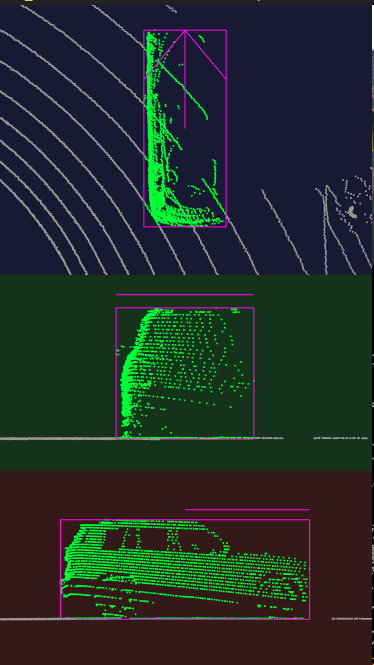
\includegraphics[height=4cm]{./figures/reg-ref-3d}
		\caption{}\label{fig:box-ref}
	\end{subfigure}\hfill
	~
	\begin{subfigure}[t]{0.18\linewidth}
		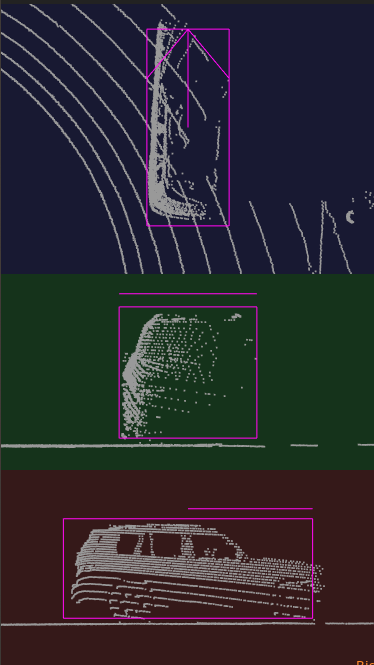
\includegraphics[height=4cm]{./figures/reg-input-3d}
		\caption{}\label{fig:box-source}
	\end{subfigure}\hfill
	~
	\begin{subfigure}[t]{0.18\linewidth}
		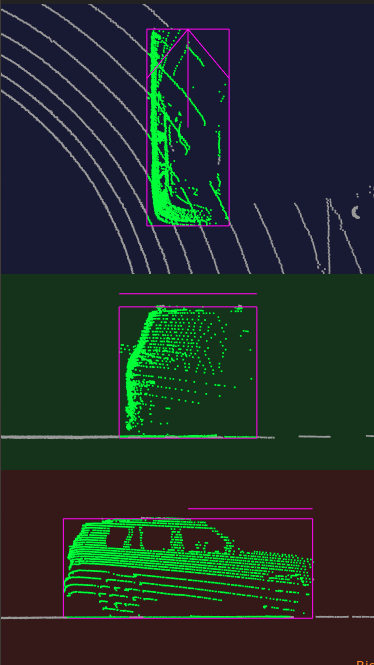
\includegraphics[height=4cm]{./figures/reg-result-3d}
		\caption{}\label{fig:box-output}
	\end{subfigure}\hfill
	~
	\begin{subfigure}[t]{0.18\linewidth}
		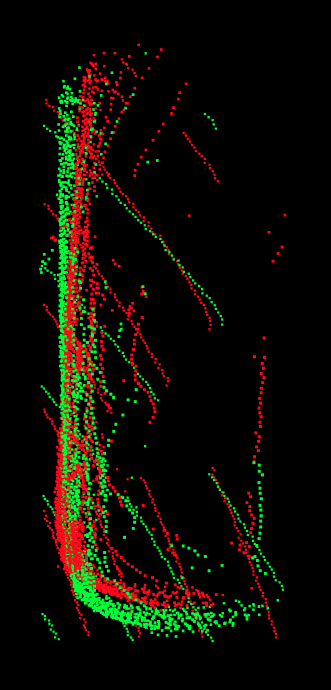
\includegraphics[height=4cm]{./figures/reg-input}
		\caption{}\label{fig:reg-input}
	\end{subfigure}\hfill
	\caption{
		An illustration of registration based annontation transfer. (a) The reference object and its bounding box. (b) The object in another frame with an initial bounding box. (c) The adjusted bounding box using our transfer algorithm. (d) The input of the registration algorithm consisting of two set of piont clouds from (a) and (b).}		
	\label {fig:annotation-transfer}
\end{figure}

\textbf{Annotation transfer among frames}. 
AD datasets are often organized in terms of data streams \cite{Caesar2019nuScenesAM,Patil2019TheHD,lyft2019}. Each stream consists of a sequence of data frames. 
There are many similarities between neighboring frames, which makes it possible to transfer annotations among them. 
Annotation results of one frame could be directly copied to the next frame directly and then adjustments are performed by users \cite{Zimmer20193DBA}.
Those box adjusting algorithms can use the object sizes estimated from previous frames \cite{Wang2019LATTEAL}. 
Our system utilizes a 3D data registration algorithm \cite{Yang2016GoICPAG} to automatically adjust box poses using the sizes and orientations of objects acquired from previous frames,
which can produce accurate annotation results in most cases.

The automatic annotation transfer needs a 3D object tracking algorithm to build the correspondence between reference objects and target objects from different frames. 
The registration algorithm is then used to compute the relative geometric transform between the reference and target objects, 
and the bounding boxes in the target frame will be adjusted accordingly.
If there is no 3D object tracking algorithm, a user needs to first select a reference box in the source frame, and copy \& paste it at an appropriate position (overlapping with the target object) in the target frame. 
The relative geometric transform between the reference and target objects will be computed and the bounding box in the target frame will be adjusted accordingly.
The reference and target objects are cropped out and all their points are transformed to the corresponding bounding box coordinates systems automatically
before feeding them into the registration algorithm.

Fig.~\ref{fig:annotation-transfer} illustrates an example of annotaton transfer, whose performance relies on the effectiveness of the registration algorithm. 
The registration works well when the orientations of reference and target objects have small deviations.

Given the reference and target objects (denoted by $\mathcal{R}$ and $\mathcal{T}$, respectively) and their bounding boxes ($b_r$; $b_t$), a registration algorithm aims to find the transform $T$ to match $\mathcal{T}$ with $\mathcal{R}$, minimizing a distance function $dist(T(\mathcal{T}); \mathcal{R} )$.

We describe the points of $\mathcal{R}$; $\mathcal{T}$ in their corresponding bounding box coordinate systems, $B_r$ and $B_t$, and the world coordinate system, $B_w$. 
Note that the box is identical to the box coordinates system (i.e. $b_r$ is identical to $B_r$) since we only concern the orientation (correspond to 3 axes) and position
(correspond to the origin point) of the box.

Assume a point of $t \in \mathcal{T}$ corresponds to a point of $r \in \mathcal{R}$ after the registration, then we will have
\begin{align}
T t^{B_t} &= r^{B_r}\\
T B_t^{-1}t^{B_w} &= r^{B_r} \label{eq:eq1}
\end{align}
where $r^{B_r}$ means a point of $r$ represented in the $B_r$ coordinate system. If the new coordinate system of $\mathcal{T}$ is denoted as $B'_t$, then we will have
\begin{align} 
t^{B'_t} &= r^{B_r}\\
(B'_t)^{-1}t^{B_w} &= r^{B_r} \label{eq:eq2}
\end{align}
From Eq. (2) and Eq. (4), we have
\begin{align}
{B'_t} & = (T B_t^{-1})^{-1}\\
& = B_t T^{-1} \label{eq:eq5}
\end{align}

The annonation transfer algorithm and crop and transform algorithms are summarized in Algorithm~\ref{alg:anno-trans}.

\begin{algorithm}
	\caption{Annotation Transfer Algorithm.}
	\label{alg:anno-trans}
	
	\SetAlgoLined
	\KwIn{reference and target point cloud $\mathcal{P}_r,\mathcal{P}_t \in \mathbb{R}^{n \times 3}$; 
		reference box $b_r=(p_r, s_r, r_r)$; initial position $p_t$ of target box, where $p,s,r \in \mathbb{R}^3$ means  position, scale and rotation, respectively, rotation is represented by Euler angles; 
		 }
	\KwOut{target box $b_t$}
	
	\nl initialize target box $b_t = (p_t,s_r,r_r)$\;
	\nl compute points of reference object $\mathcal{R}$ represned in coordinate system $B_r$ by calling Algorithm.~\ref{alg:crop-trans} with input $\mathcal{P}_r$ and $b_r$\;
	\nl compute points of target object $\mathcal{T}$ represned in coordinate system $B_t$ by calling Algorithm.~\ref{alg:crop-trans} with input $\mathcal{P}_t$ and $b_t$\;
	\nl compute relative rotation $\rho$ and translate $\tau$ by registering $\mathcal{T}$ to $\mathcal{R}$ with registration algorithm \cite{Yang2016GoICPAG} \;
	\nl compute $\tau'$ by transform $\tau$ from box coordinate system $B_t$ into world coordinate system $B_w$\;
	\nl	by using Eq.~(\ref{eq:eq5}), compute $b_t = (p_t-\tau', s_r, r_r-\rho)$\;
	\nl return $b_t$\;
	
\end{algorithm}
\begin{algorithm}
	\caption{Crop and Transform Algorithm.}
	\label{alg:crop-trans}
	
	\SetAlgoLined
	\KwIn{point cloud $\mathcal{P} \in \mathcal{R}^{n \times 3}$; box $b=(p,s,r)$ where $p,s,r \in \mathbb{R}^3$ means  position, scale and rotation, respectively, rotation is represented by Euler angles.}
	\KwOut{ set of points $R \in \mathbb{R}^{m \times 3}$ in box $b$, represented in $b$'s box coordinate system.}
	\nl initialize $R = \emptyset $ \;
	\nl \For {point $x$ in $\mathcal{P}$}{
	\nl 	compute $x'$ by representing $x$ in $b$'s coordinate system\;
	\nl 	\If{$x'$ lies inside box $b$} 
				{
	\nl			append $x'$ into $R$
				}
	}
	\nl return $R$\;
	
\end{algorithm}

\section{Results And Discussions}
\label {sec:results}

Generally speaking, it is hard to evaluate an 3D point cloud annotation platform as there are no standard benchmark metrics.
In this work, we use KITTI \cite{Geiger2012CVPR} and SUSTech SCAPES to test the developed POINTS.
The whole evaluation contains three parts:
1) Annotation error checking effieicency. We use the KITTI dataset\cite{Geiger2012CVPR} to test POINTS's new visualization functionalities which help users to check the annotation errors.
2) Annotation efficiency. We compare POINTS and PointAtMe \cite{pointatme} in the terms of annotation errors and speeds.
3) Annotation transfer quality. We use four target frames for annotation transfer from one reference frames with three types of objects: car, rider, and bus.


\subsection{Annotation Error Checking Efficiency}
Examples from the KITTI 3D Object Detection dataset \cite{Geiger2012CVPR} are used to demonstrate the effectiveness and efficiency of POINTS in checking annotation errors. 
The same examples are chosen as shown in Fig. 5 of \cite{pointatme}. 
Although our platform supports all 9 degrees of freedom (DOFs) for 3D bounding boxes, only 7 DOFs (without pitch and tilt) are labeled in the KITTI dataset.
Therefore, we only test those examples with 7 DOFs.
Fig.~\ref{fig:annocheck} shows examples of annotation errors checking with the KITTI 3D object detection dataset using POINTS. 
It contains the top, front, side views and photo context of two cars and a pedestrian.
It can be seen that with the help of the 4 sub-views and object coloring (Section\ref{sec:visualization}) 
annotation errors, such as front mirrors, hands, part of cars outside the bounding boxes and the margins between bounding boxes and objects
can be quickly identified by just selecting the objects from one to another (Section~\ref{sec:navigation}).
Meanwhile, tracking IDs can also be easily checked with the help of the functionalities of object locking and stream playing (Section III-B).

\begin{figure}
	\centering
	\begin{subfigure}{0.3\linewidth}
		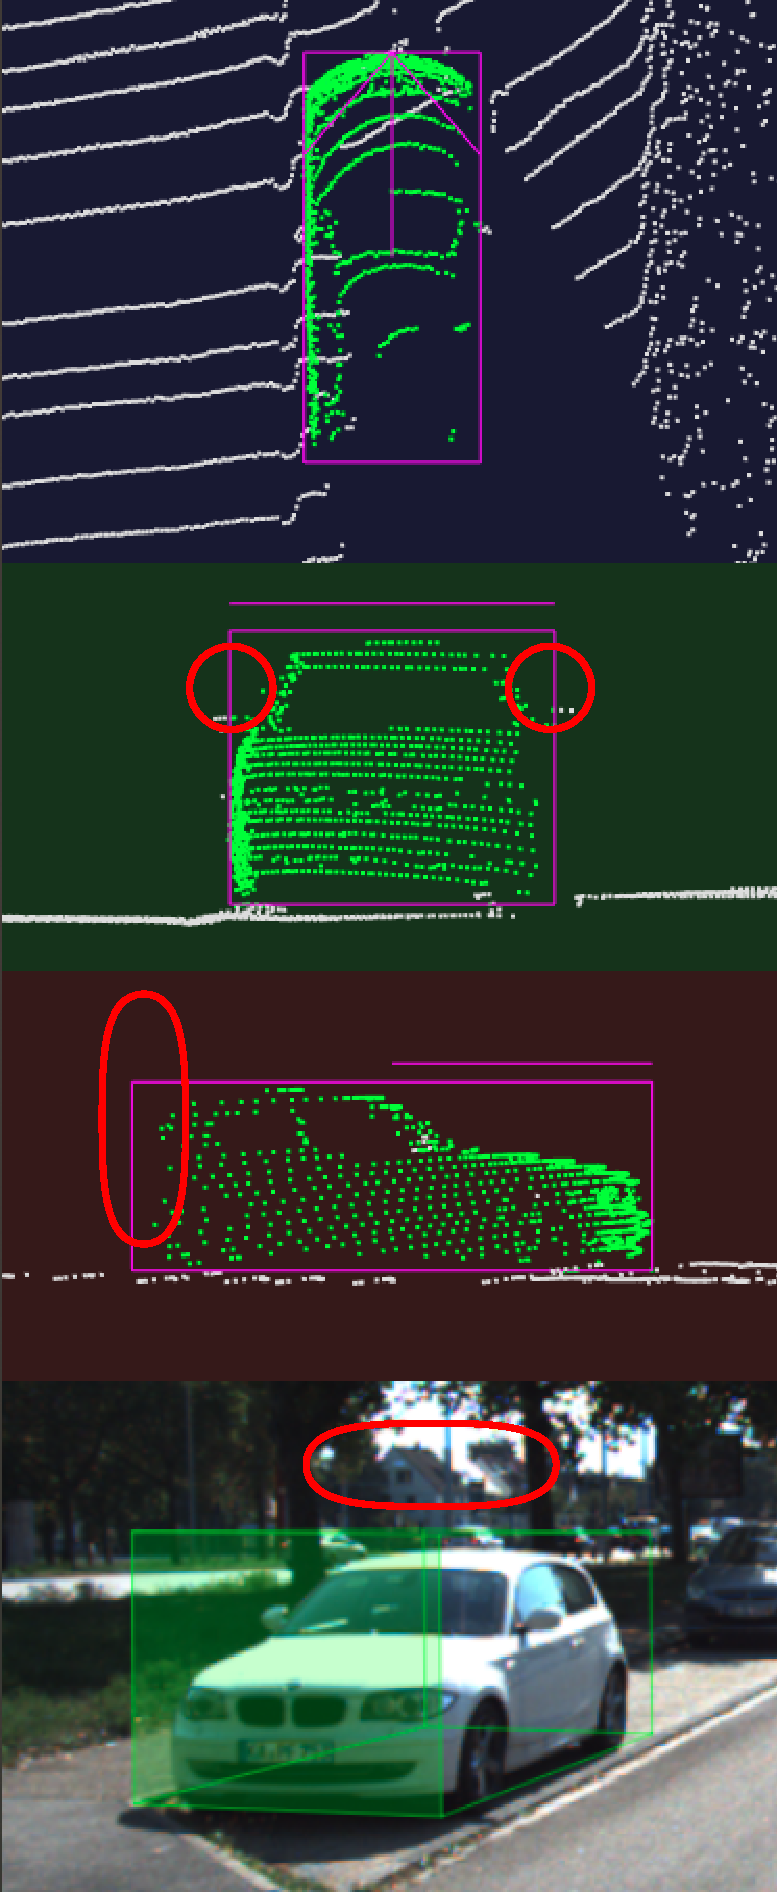
\includegraphics[scale=0.2]{./figures/annocheck-0}
		\caption{}
	\end{subfigure}
	~
	\begin{subfigure}{0.3\linewidth}
		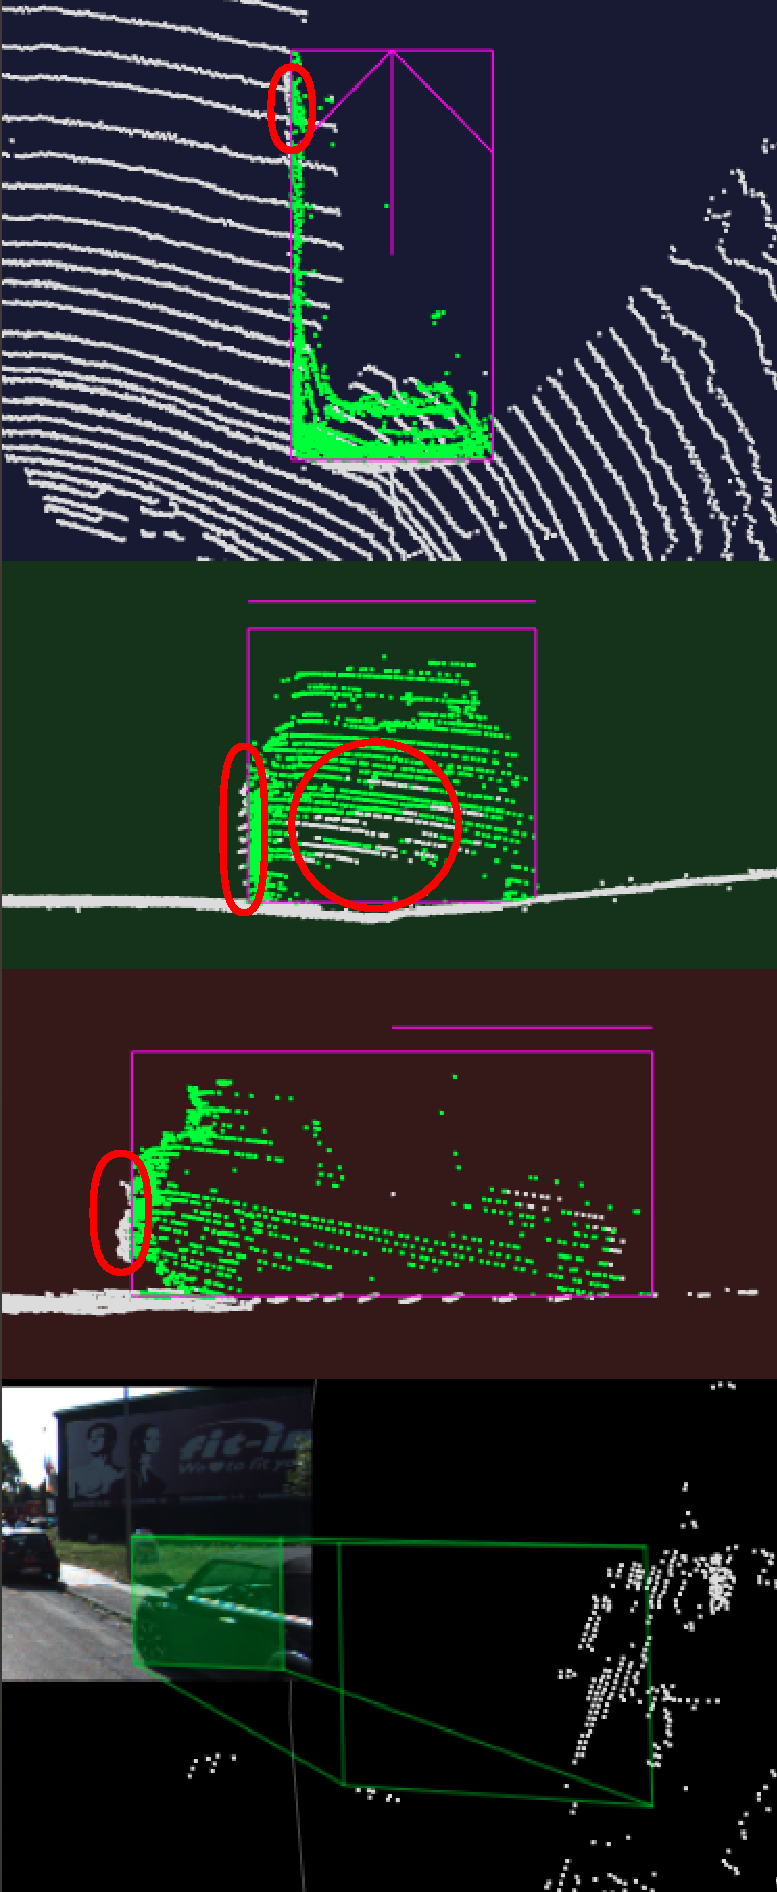
\includegraphics[scale=0.2]{./figures/annocheck-1}
		\caption{}
	\end{subfigure}
	~
	\begin{subfigure}{0.3\linewidth}
		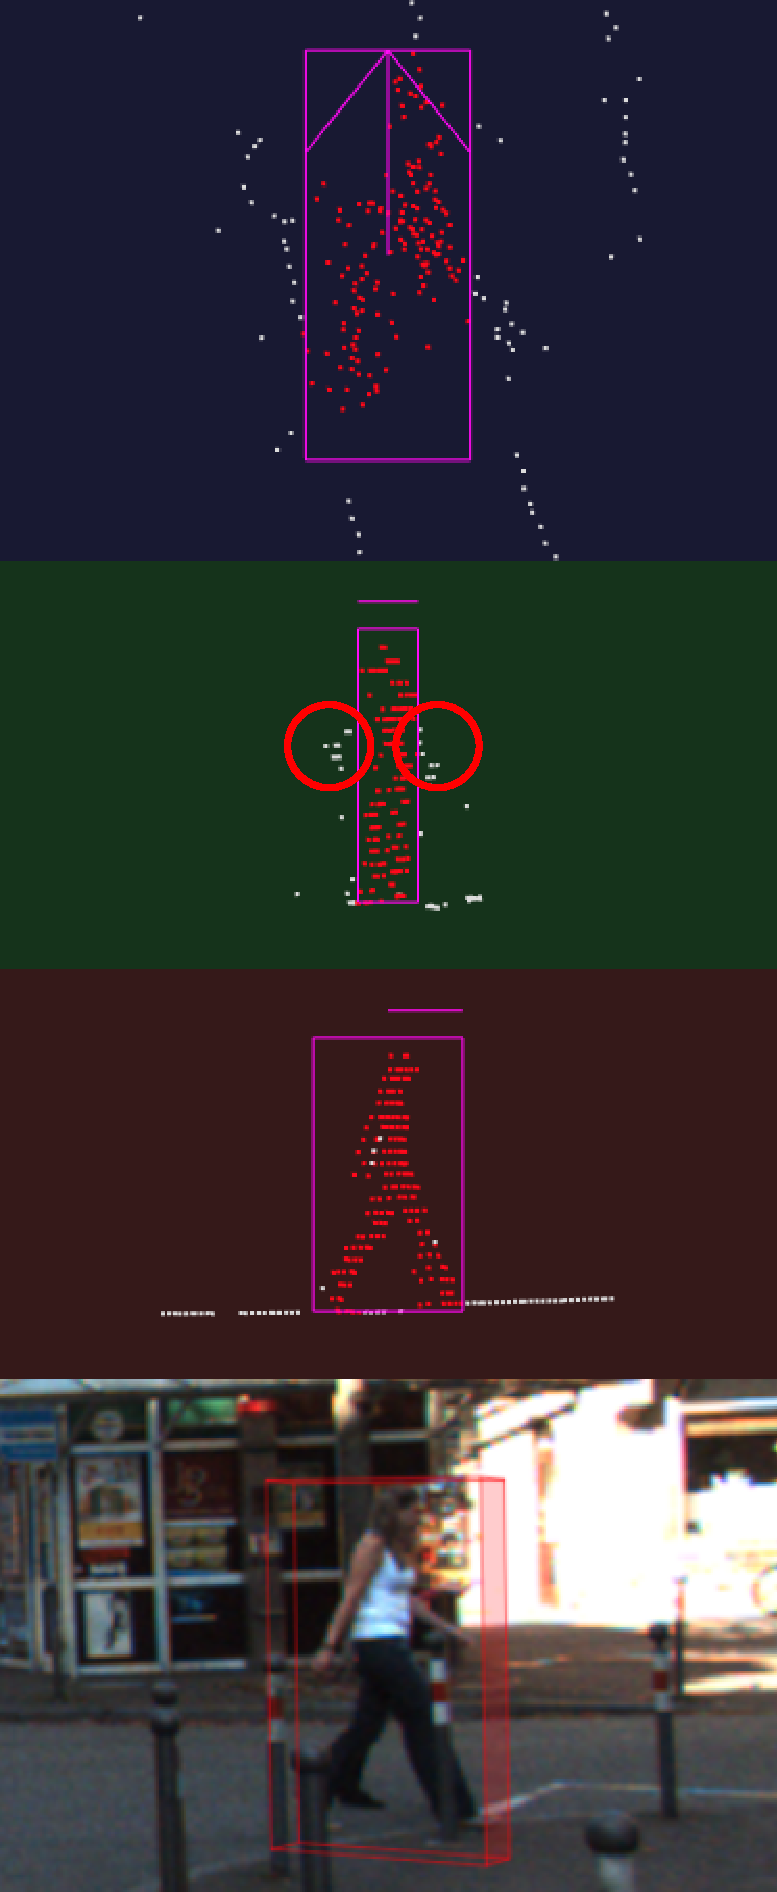
\includegraphics[scale=0.2]{./figures/annocheck-2}
		\caption{}
	\end{subfigure}
	
	\caption{
	An illustration of annotation errors checking with the KITTI 3D object detection dataset using POINTS. 
	(a) The top, front, side views and photo context of a car, 
	where two front mirrors are out of the bounding box, and the bounding box has back and top margins over the car. 
	(b) The top, front, side views and photo context of a car,
	where one front mirror, the left side and the back part of the car are out of the bounding box.
	(c) The top, front, side views and photo context of a pedestrian,     
	where the two hands are out of the bounding box.}
	\label{fig:annocheck}
\end{figure}


\subsection{Annotation Efficiency}

Annotation efficiency can be measured by annotation accuracy and speed \cite{pointatme} \cite{Zimmer20193DBA}. POINTS aims to maximize the annotation accuracy within the minimum time.
As original KITTI labels are not suited as ground truth due to their accuracy not high enough, 
we carefully annotated some KITTI scenes and use the results as the ground truth \cite{pointatme}.
Three users are employed to annotate the same set of data after a few hours of practicing. 
For each user we measure the average annotation time (seconds) per object and average annotation errors per object.
For a perfect annotation, all the points belonging to an object should be inside the bounding box and otherwise outside. 
Three metrics are used: 1) the number of error points per object, 
2) the relative number of False Positive (FP) points per object, and 
3) the relative number of False Negative (FN) points per object. 

As shown in Table~\ref{tab:annotation-evaluation}, the annotated accuracy obtained by those unexperienced users using POINTS are very close to the ground truth,
much higher than using PointAtMe (baseline) with less than half of the annotation time. 
The success should attribute to the developed techniques such as smart box initialization, interactive box fitting and convenient visualization modules. 
Users only need to ensure the points of one object are all inside one 2D rectangle initially, and do not need to refine the 3D bounding box by themselves, 
reducing many human errors. 
Meanwhile, the annotation speed is also improved by more than two times compared to the baseline. 
It can be seen that POINTS can really help unexperienced users to achieve high annotation efficiency. 



\begin{table}[h]
	\centering
	\caption{A comparison of annotation efficiency between POINTS and PointAtMe using the KITTI dataset.}
	\label{tab:annotation-evaluation}
	\begin{tabular}{|l|c|c|c|c||c|c|c|c|}
		\hline
		\textbf{Method} & \textbf{Ours (POINTS)} & \textbf{PointAtME\cite{pointatme}} \\
		\hline
		\hline
		Time/Object (sec.) & 24 $\pm$ 6 & 55.2 $\pm$ 12.1\\
		\hline
		%Undo/Object & - & 0.42 $\pm$ 0.43\\
		%\hline
		Errors (Points/Object) & $<$1 & 28.7 $\pm$ 5.1\\
		\hline
		FP ratio / Object & 0 & 7.16\%\\
		\hline
		FN ratio / Object & $<$1\% & 3.27\%\\
		\hline
	\end{tabular}
\end{table}


\subsection{Annotation Transfer Quality}
Our private dataset (SUSTech SCAPES) is used to evaluate the annotation transfer quality among five frames at 0s, 0.5s, 1s, 1.5s, and 2.5s.  
We choose three scenarios with different object types: 
1) scenario 1: a car moving away from the ego-car along a straight line while the ego-car waiting for the red light, 
2) scenario 2: a rider crossing the road while the ego-car approaching to the rider, and 
3) scenario 3: a bus and the ego-car both moving forward on the same road with reverse directions. 
The frame at 0s is chosen as the reference frame, and hence reference objects have the largest number of points. 
Table III shows that the distance between the ego-car and the target object increases as the time goes by, 
because the numbers of 3D data points of those objects decrease accordingly. 
For example, in scenario 3, the bus only has 173 data points in the frame of 2.5s, 7.4\% of the reference object's 2327 data points in the frame of 0s.
Elaborate annotation results of those scenarios are chosen as the ground truth.
The Error Points Per Object and the relative FN points number per object are used to evaluate the annotation transfer quality.

The results of transfer annotation are shown in Table~\ref{tab:transfer-evaluation} and Fig.~\ref{fig:anno-transfer}.
It can be seen that 
for scenario 1, the annotation transfer errors of the car are less than 2.7\%, with the relative number of FN points of 1.7\%;
for scenario 2, the annotation transfer errors of the rider are 0, with the relative number of FN points of 0\%;
for scenario 3, the annotation transfer errors of the bus are less than 0.5\%, with the relative number of FN points of 0.28\%  
Compared with Table II, it can be seen that the accuracy of transfer annotation is lower than manual annotations, 
but still higher than baseline (although we used a different dataset).
With the help of such a annotation transfer technique, each object in a data stream needs only almost once manual annotation at the begining. 
Such a technique can also help solve the problem of distant or occluded objects when the number of data points are very sparse. 
We believe that this technique is complementary to other existing annotation transfer algorithms, such as direct pasting and linear interpolation, 
and if integrated with tracking algorithms POINTS could improve the annotation efficiency further.


\begin{table}[h]
	\centering
	\caption{Annotation transfer results among five frames for three scenarios using POINTS with the SUSTech SCAPES dataset.}
	\label{tab:transfer-evaluation}
	\resizebox{1.0\linewidth}{!}{
	\begin{tabular}{|c|r|c|c|c|c|c|c|c|}
		\hline
		 \#& \textbf{Type} & \textbf{Ref. Obj.}&\textbf{0.5s} & \textbf{1s} & \textbf{1.5s}& \textbf{2.5s} &\textbf{Err/Obj} & \textbf{FN Ratio}\\
		\hline
		\hline
		 1 & Car &-/1958& 15/1387 & 25/935 & 19/677 &  1/389 & 15 & 1.7\% \\
		\hline
  		 2 & Rider &-/329& 0/240 & 0/190 & 0/149 &  0/94 & 0 & 0\\
		\hline
  		 3 & Bus &-/2327& 5/1208 & 3/656 & 1/396 &  0/173 & 2.25& 0.28\%\\
\hline
	\end{tabular}
	}
\begin{tabular}{p{\linewidth}}
	The value is in the form of Error points/Total points. “Ref. Obj.” means the reference object (i.e. the manually annotated object). 
	The “Err/Obj” and “FN” are the same as in Table II.	
\end{tabular}
\end{table}

\begin{figure}[h]
	\centering
	\begin{subfigure}{0.16\linewidth}
		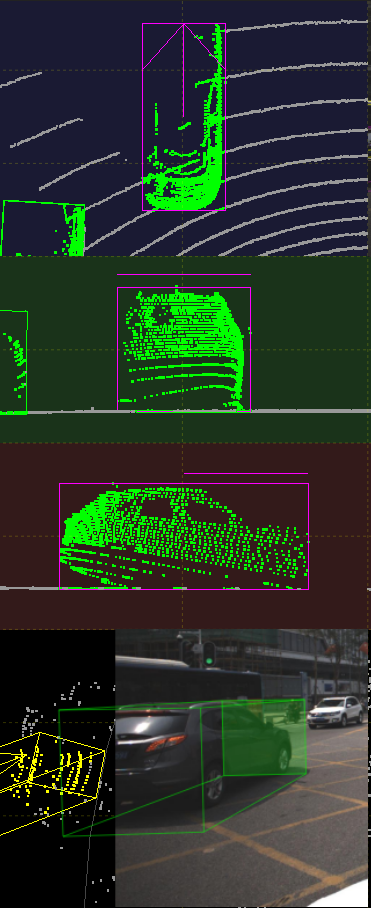
\includegraphics[scale=0.12]{./figures/transfer/car-ref}
		\caption{}
	\end{subfigure}
	~
	\begin{subfigure}{0.16\linewidth}
		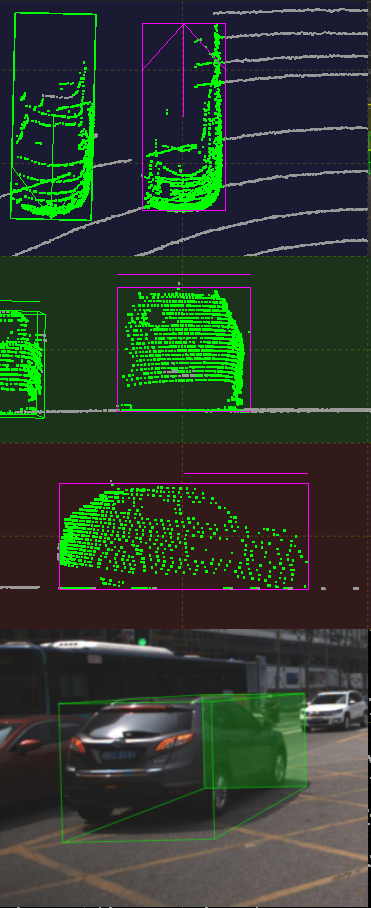
\includegraphics[scale=0.12]{./figures/transfer/car-1}
		\caption{}
	\end{subfigure}
	~
	\begin{subfigure}{0.16\linewidth}
		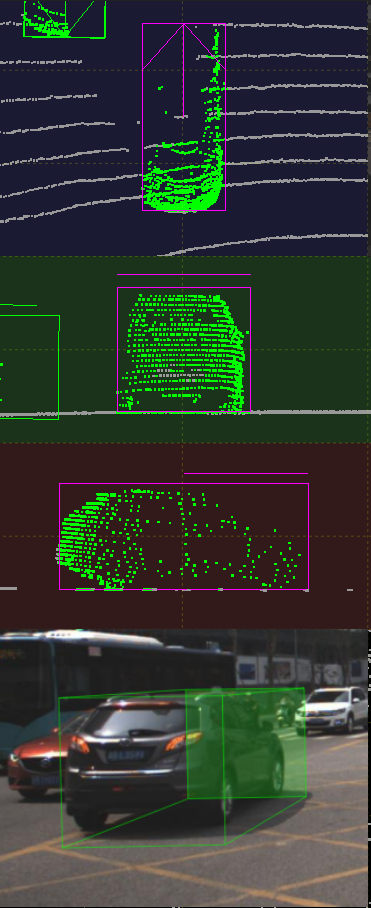
\includegraphics[scale=0.12]{./figures/transfer/car-2}
		\caption{}
	\end{subfigure}
		~
	\begin{subfigure}{0.16\linewidth}
		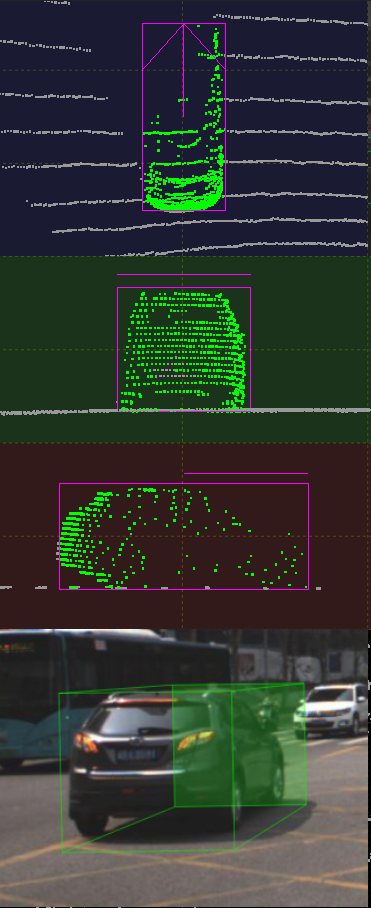
\includegraphics[scale=0.12]{./figures/transfer/car-3}
		\caption{}
	\end{subfigure}
	~
	\begin{subfigure}{0.16\linewidth}
		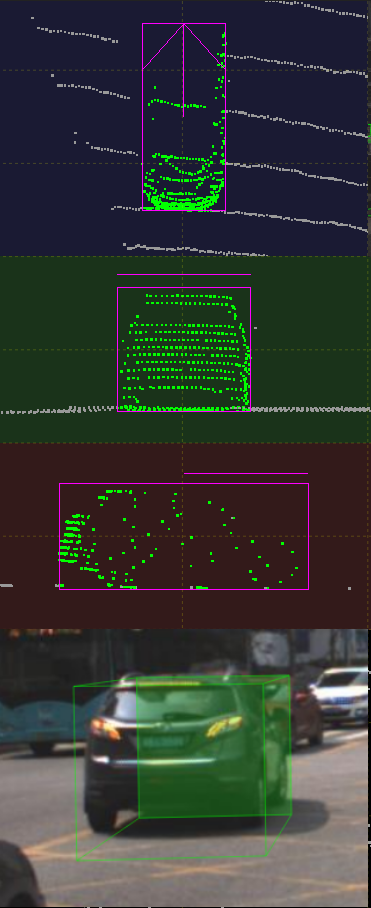
\includegraphics[scale=0.12]{./figures/transfer/car-5}
		\caption{}
	\end{subfigure}

	\begin{subfigure}{0.16\linewidth}
		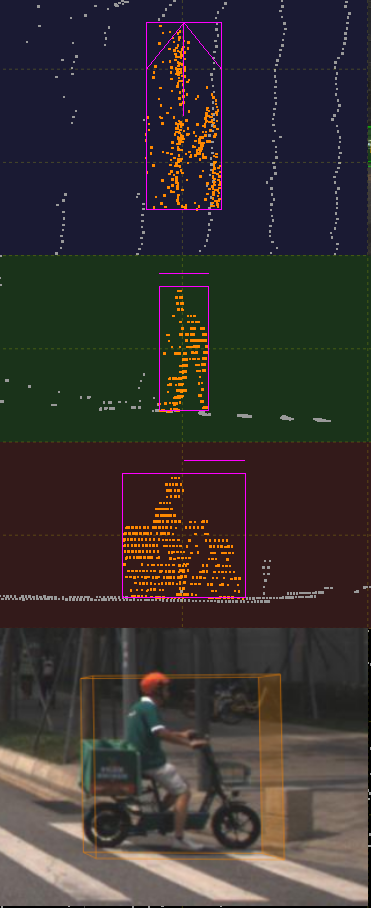
\includegraphics[scale=0.12]{./figures/transfer/rider-ref}
		\caption{}
	\end{subfigure}
	~
	\begin{subfigure}{0.16\linewidth}
		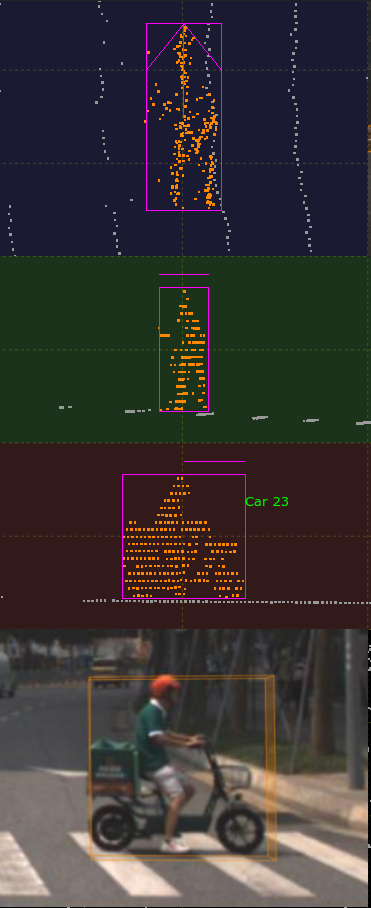
\includegraphics[scale=0.12]{./figures/transfer/rider-1}
		\caption{}
	\end{subfigure}
	~
	\begin{subfigure}{0.16\linewidth}
		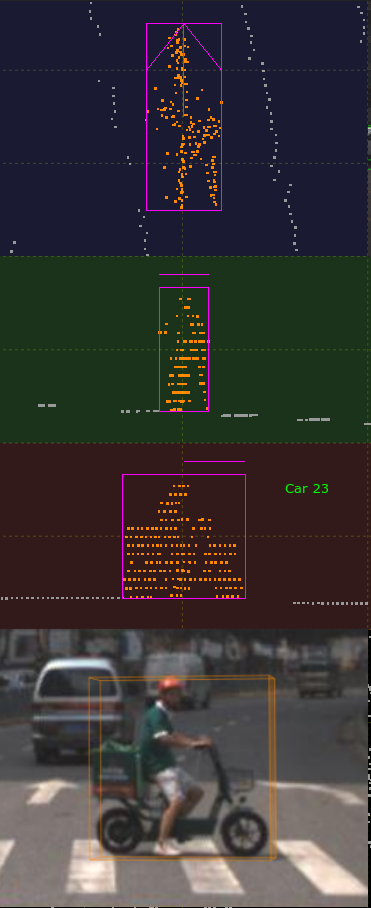
\includegraphics[scale=0.12]{./figures/transfer/rider-2}
		\caption{}
	\end{subfigure}
	~
	\begin{subfigure}{0.16\linewidth}
		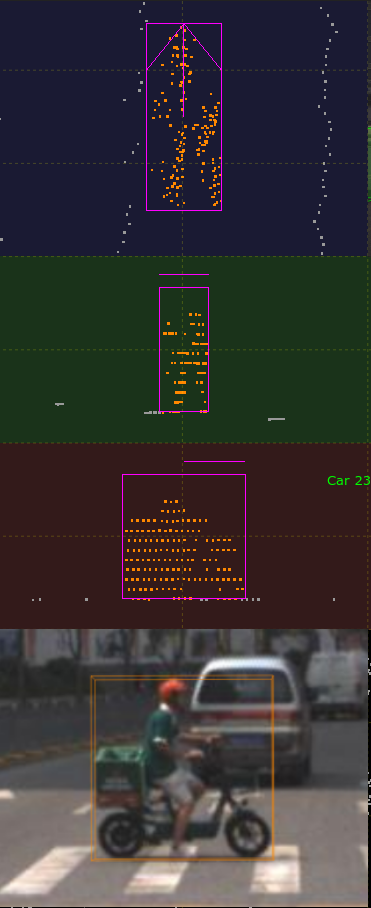
\includegraphics[scale=0.12]{./figures/transfer/rider-3}
		\caption{}
	\end{subfigure}
	~
	\begin{subfigure}{0.16\linewidth}
		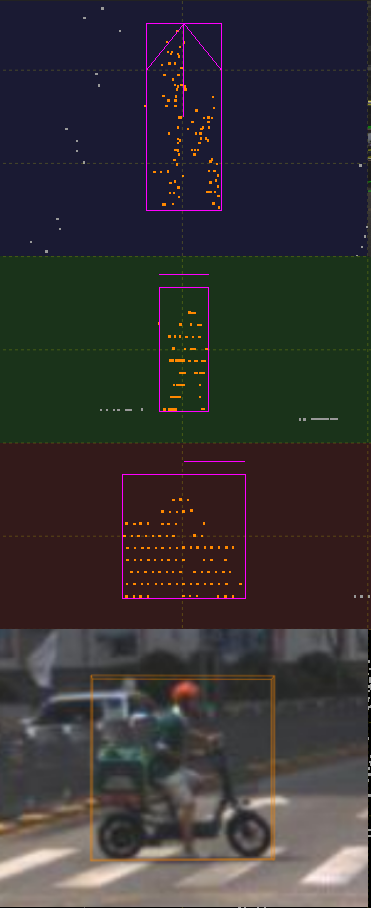
\includegraphics[scale=0.12]{./figures/transfer/rider-5}
		\caption{}
	\end{subfigure}
	
	
	\begin{subfigure}{0.16\linewidth}
		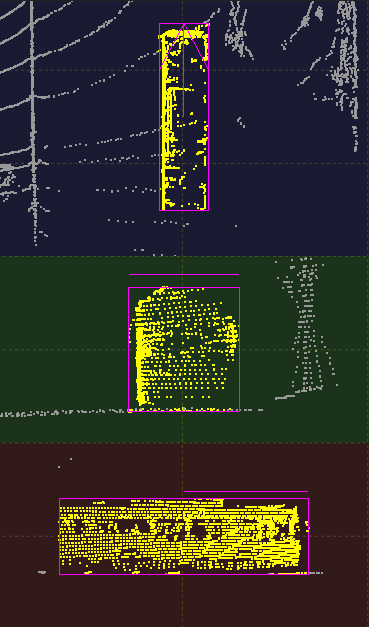
\includegraphics[scale=0.12]{./figures/transfer/bus-ref}
		\caption{}
	\end{subfigure}
	~
	\begin{subfigure}{0.16\linewidth}
		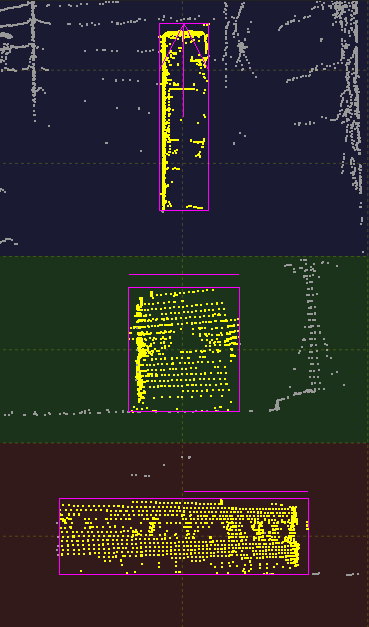
\includegraphics[scale=0.12]{./figures/transfer/bus-1}
		\caption{}
	\end{subfigure}
	~
	\begin{subfigure}{0.16\linewidth}
		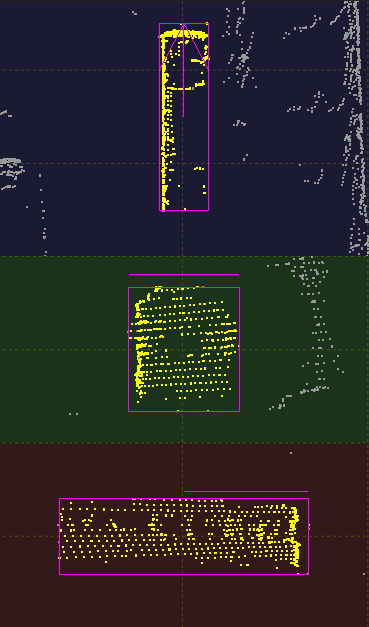
\includegraphics[scale=0.12]{./figures/transfer/bus-2}
		\caption{}
	\end{subfigure}
	~
	\begin{subfigure}{0.16\linewidth}
		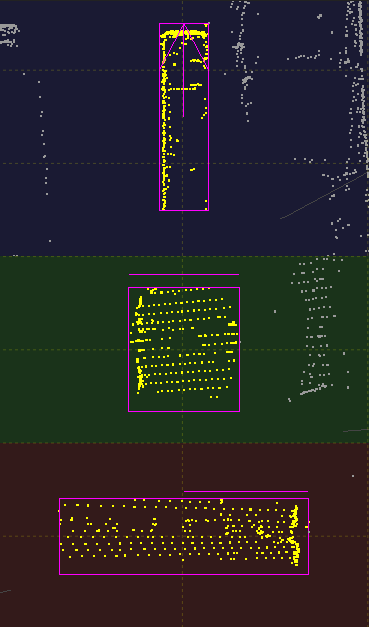
\includegraphics[scale=0.12]{./figures/transfer/bus-3}
		\caption{}
	\end{subfigure}
	~
	\begin{subfigure}{0.16\linewidth}
		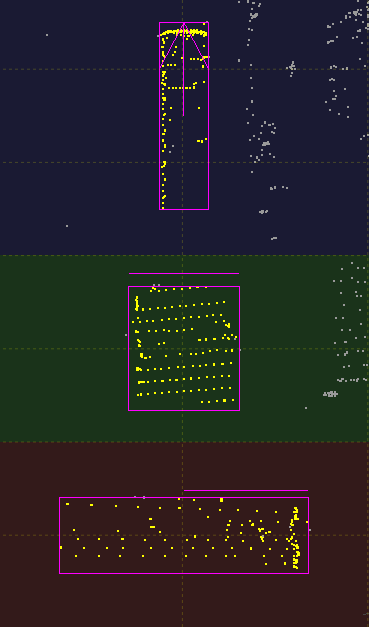
\includegraphics[scale=0.12]{./figures/transfer/bus-5}
		\caption{}
	\end{subfigure}
	\caption{Annotation transfer results among five frames for three scenarios using POINTS with the SUSTech SCAPES dataset. The three rows correspond to 3 scenarios. The left column (a,f,k) are references frames whose bounding boxes are annotated manually, the remaining columns are frames of 0.5s, 1s, 1.5s and 2.5s, respectively, whose bounding boxes are generated by the annotation transfer algorithm of POINTS. For scenarios 1 and 2 (a-j), the top, front, side views and photo context are shown, for scenario 3 (k-o) only top, front, side views are shown. In scenario 1 (a-e), the back part (b-d) and the front mirror (e) of the car are out of the bounding box. In scenario 2 (f-j), there is no errors. In scenario 3 (k-o), the back part (l, m) and the front mirror (m, n) of the bus are out of the bounding box.}
	\label{fig:anno-transfer}
\end{figure}


\section{CONCLUSION}
\label{sec:conclusions}

In this paper, we have presented a framework for developing portable 3D point cloud iterative annotation platform systems (POINTS) for AD applications. 
A number of important data visualization modules and interative operation tools, as well as supporting algorithms, have been specifically introduced.
The major contributions of this work include developing a series of enhanced data visulization modules, new interactive tools, and a registration-based annotation transfer method to acheve high-accuracy and high-efficiency human-in-the-loop 3D data annotation.
The source codes of the developed SUSTech POINTS are available on Github for public access.
Compred with PointAtMe, the proposed POINTS can achieve much lower annotation errors in shorter annotation time, tested with KITTI, nuScenes, and SUSTech SCAPES datasets. 
The developed annotation transfer method can tranfer annotations from one frame to multiple frames with errors of no more than 3\%.
The future work includes integrating more AI-based algorithms, such as 3D object tracking algorithms, with our annotation platform (POINTS) to achieve more automatic annontation functionalities with high quality.




\addtolength{\textheight}{-12cm}   % This command serves to balance the column lengths
                                  % on the last page of the document manually. It shortens
                                  % the textheight of the last page by a suitable amount.
                                  % This command does not take effect until the next page
                                  % so it should come on the page before the last. Make
                                  % sure that you do not shorten the textheight too much.

%%%%%%%%%%%%%%%%%%%%%%%%%%%%%%%%%%%%%%%%%%%%%%%%%%%%%%%%%%%%%%%%%%%%%%%%%%%%%%%%



%%%%%%%%%%%%%%%%%%%%%%%%%%%%%%%%%%%%%%%%%%%%%%%%%%%%%%%%%%%%%%%%%%%%%%%%%%%%%%%%



%%%%%%%%%%%%%%%%%%%%%%%%%%%%%%%%%%%%%%%%%%%%%%%%%%%%%%%%%%%%%%%%%%%%%%%%%%%%%%%%
\begin{comment}


\section*{APPENDIX}

\subsection{Raw data orgnization}
In server, the raw data is organized by scenes, the directory structure is as in Fig.~\ref{fig:data-dir}.

\begin{figure}

	\dirtree{%
		.1 data.
		.2 scene1.
		.3 lidar.
		.4 frame0000.pcd.
		.4 ....
		.3 image.
		.4 left-camera.
		.5 frame0000.png.
		.5 ....
		.4 front.
		.5 frame0000.png.
		.5 ....
		.4 ....
		.3 calib.
		.4 left-camera.json.
		.4 front.json.
		.4 ....
		.3 label.
		.5 frame0000.json.
		.5 ....
		.2 scene2.
		.3 ....
		.2 ....
	}
	\caption{Raw data organization. The `label` folder is used to store annotation result. the `calib` folder stores lidar-camera calibration parameters, which is optional but requrired for 3d-2d fusion features. We list 3 cameras as an example, more cameras are also supported.}
	\label{fig:data-dir}
\end{figure}


\subsection{Operation summary}
\label{app:operations}
Table~\ref{table:keyboard_mainview} shows operations applicable in main view, Table~\ref{table:keyboard_subview} show operations applicable in side sub-views.

\begin{table}[h]
	\caption{Operations on main-view}
	\label{table:keyboard_mainview}
	\begin{center}
		\begin{tabular}{|c|l|}
			\hline
			\textbf{Key} & \textbf{Function}\\
			\hline
			1 & select previous object\\
			\hline
			2 & select next object\\
			\hline
			3 & previous frame\\
			\hline
			4 & next frame\\
			\hline
			r & rotate counterclockwise(yaw)\\
			\hline
			f & rotate clockwise(yaw)\\
			\hline
			t & reset box\\
			\hline
			g & reverse direction (yaw angle)\\
			\hline
			v & switch editing mode(Fig.~\ref{fig:box-mouse-edit})\\
			\hline
			Ctrl+s & save\\
			\hline
			Ctrl+c & copy reference box (\ref{semi-auto-anno})\\
			\hline
			Ctrl+z & undo\\
			\hline
			Ctrl+y & redo\\
			\hline
			Left drag & rotate view\\
			\hline
			Right drag & pan view\\
			\hline
			Wheel up & zoom in\\
			\hline
			Wheel down & zoom out\\
			\hline
			Ctrl+Left Drag (on main view)& mark points\\
			\hline
			Ctrl+Left click (on photo context)& draw polygon\\
			\hline
		\end{tabular}
	\end{center}
\end{table}


\begin{table}[h]
	\caption{Operations on sub-views}
	\label{table:keyboard_subview}
	\begin{center}
		\begin{tabular}{|c|l|c|l|}
			\hline
			\textbf{Key} & \textbf{Function}\\			
			\hline
			a & move left\\
			\hline
			s & move down\\
			\hline
			d & move right\\
			\hline
			w & move up\\
			\hline
			q & rotate left\\
			\hline
			e & rotate right\\
			\hline
			q & rotate left\\
			\hline
			e & rotate right\\
			\hline				
			Ctrl-q & rotate left with boundary aware\\
			\hline
			Ctrl-e & rotate right with boundary aware\\
			\hline
			Drag box border/corner & resizing box\\
			\hline
			Drag direction line & rotate box\\
			\hline
			Drag box border/corner with Ctrl hold & resizing box with auto-shrink\\
			\hline
			Drag direction line with Ctrl hold& rotate box with boundary aware\\
			\hline
			Drag box center & move box\\
			\hline
			Double click box border/corner & auto-shrinking\\
			\hline
			Double click box center & auto-shrinking all borders\\
			\hline
			Double click direction line& rotate upside-down (180 degree)\\
			\hline
		\end{tabular}
	
		 {\raggedright Note that all operation effects are relative to current sub-view.\par}
		 
	\end{center}
\end{table}
\section*{ACKNOWLEDGMENT}


\end{comment}

%%%%%%%%%%%%%%%%%%%%%%%%%%%%%%%%%%%%%%%%%%%%%%%%%%%%%%%%%%%%%%%%%%%%%%%%%%%%%%%%


\bibliographystyle{IEEEtran}
\bibliography{MyReference}
\end{document}
